\chapter{Scientific Background}
\label{chap:scientific}

\section{Conventions}
\subsection{Reference system}

In what follows, we will make use of a right-handed coordinate system, where the positive \textit{x}-axis points towards the \textit{front}, the positive \textit{y}-axis points towards the \textit{left}, and the positive \textit{z}-axis points towards the \textit{zenith} (North Pole).

Any position in the unit sphere may be described in spherical coordinates by two angles: the \textit{inclination} angle $\vartheta$, which accounts for the aperture with respect to the \textit{z}-axis, and the \textit{azimuth} angle $\varphi$, which represents the counter-clockwise angle with respect to the \textit{x}-axis from the top-view. 
The value ranges are $0 \leq \vartheta \leq \pi$ for the inclination, and $0 \leq \varphi \leq 2\pi$ for the azimuth. 

Table~\ref{tab:cartesian} shows the spherical coordinate values for some reference points on the unit sphere.
Notice that the poles ($\vartheta = �\pi$) are a special case for the spherical coordinate system -- in that case, the azimuth angle is not defined. \\


\begin{table}[!htbp]
\centering
\caption{Cartesian and spherical representation of characteristic points along the unit sphere.}
  \begin{tabular}{cccc}
  \toprule
    Position & Cartesian & $\vartheta$ & $\varphi$ \\
\midrule
	front & $[1, 0, 0]$ & $\pi/2$ & $0$ \\
	back & $[-1, 0, 0]$ & $\pi/2$ & $\pi$ \\
	left & $[0, 1, 0]$ & $\pi/2$ & $\pi/2$ \\
	right & $[0, -1, 0]$ & $\pi/2$ & $-\pi/2$ \\
    \textit{zenith} & $[0, 0, 1]$ & $0$ & * \\
    \textit{nadir}  & $[0, 0, -1]$ & $\pi$ & * \\
    \bottomrule
  \end{tabular}
\label{tab:cartesian}
\end{table}


The transformation between spherical and cartesian coordinate systems is given by the following relationship:
\begin{equation}
	\begin{aligned}
		x = & \cos{\varphi} \sin{\vartheta}\\
		y = & \sin{\varphi} \sin{\vartheta}\\
		z = & \cos{\vartheta}\\
	\end{aligned}
\end{equation}

The \textit{elevation} angle $\theta$ provides an alternative way of describing the relationship with respect to the \textit{z}-axis. $\theta$ is defined as  the aperture with respect to the \textit{xy}-plane, with positive values towards the positive \textit{z}-axis. The relationship between elevation and inclination angles is:
\begin{equation}
	\theta = \pi/2 - \vartheta
\end{equation}


For the sake of compactness, a point in the unit sphere will be often represented by $\Omega = (\vartheta, \varphi)$.\\

Given the periodic nature of the azimuth angle, the descriptive statistic operations applied to $\vartheta$ will refer to the $2\pi$-\textit{periodic} version or the operator; this situation does not affect the inclination/elevation coordinate.


\subsection{Nomenclature}
\todo{is this name correct? }
Throughout the Thesis, we refer to time-domain signals with lowercase, e.g. $x(t)$, with $t$ as the time index. 

Time-domain signals transformed by the Short-Time Fourier Transform (STFT) are represented with uppercase, e.g. $X(k,n)$, where $k$ is the frequency bin index, and $n$ the time frame index. 

Multichannel signals are in general denoted by a subscript variable index, usually with the letter $m$; for example, $x_m(t)$ or $X_m(k,n)$.
Signals with an integer subscript index, such as $x_0(t)$, represent a specific channel of the corresponding multichannel signal.

In the context of ambisonic, subscripts and superscripts are used in signal names with a specific meaning; check Section~\ref{sec:ambisonics} for a detailed explanation.

Vector notation is represented with boldface characters, e.g. $\bm{X}(k,n)$.  When used, the way to construct the vectors will be specified. 



\section{Spherical Harmonics}

\subsection{Definition}

Spherical harmonics are continuous functions defined on the sphere surface. Due to their mathematical properties, any spherical function can be decomposed as a combination of spherical harmonics, in what is known as the \textit{Spherical Harmonics Expansion} \cite{jarrett2017theory}.




%The spherical harmonic of \textit{order} $\ell>0$ and \textit{degree} $m$, with $|m| <= \ell$  in the direction \Omega is defined as:
Many different spherical harmonic definitions exist in the literature, with minor variations among them. In the following, we will use the real-valued, fully normalized spherical harmonics as defined by \cite{zotter2019ambisonics}: 

\begin{equation}
%ambisonics book 186
	Y_n^m(\varphi, \vartheta) = N_n^{|m|} P_n^{|m|}\cos(\vartheta) \Phi_m(\varphi), 
	\label{eq:sphericalharmonics}
\end{equation}

where the \textit{normalization factor} $N_n^m$ is:

\begin{equation}
%ambisonics book 186
	N_n^m = (-1)^m \sqrt{\frac{2n+1}{2} \frac{(n-m)!}{(n+m)!}}
\end{equation}

the \textit{Legendre polynomials} $P_n^{m}$ are defined as: 

\begin{equation}
%ambisonics book 185
	P_{n+1}^{m} =
	\begin{cases}
 		\frac{2n+1}{n-m+1} x P_n^{m},  &\text{for } n = m,  \\
 		\frac{2n+1}{n-m+1} x P_n^{m} - \frac{n+m}{n-m+1}P_{n-1}^{m} &\text{else}, \\
 	\end{cases}
\end{equation}

with $P_{n}^{n} = \frac{(-1)^n(2n)!}{2^nn!}\sqrt{1-x^{2^n}}$
and the initial term $P_{0}^{0} = 1$, 

and $\Phi_m$ is the azimuthal part of the spherical harmonics: 

\begin{equation}
%ambisonics book 176
	\Phi_m(\varphi) = \frac{1}{\sqrt{2\pi}}
	\begin{cases}
    	\sqrt{2} \sin(|m|\varphi),  &\text{for } m < 0,  \\
    	1,  & \text{for } m = 0,  \\
    	\sqrt{2} \cos(m\varphi),  & \text{for } m > 0.  \\
  	\end{cases}
\end{equation}


One of the properties of the spherical harmonics is orthonormality on the sphere surface:

\begin{equation}
	\int_{\mathbb{S}^2} Y_n^m(\varphi, \vartheta) Y_{n'}^{m'}(\varphi, \vartheta) \dif cos{\vartheta} \dif \varphi = \delta_{nn'} \delta_{mm'},
	\label{eq:orthonormality}
\end{equation}

where $\delta_{xy}$ represents the Kronecker delta operator:
\begin{equation}
	\delta_{xy} = \begin{cases}
		1,  &\text{if } x = y,\\
		0,  &\text{else}.
	\end{cases}
\end{equation}

The spherical harmonics depend on the \textit{order} $n \geq 0$ and the \textit{degree} $m$,  $|m| \leq n$ for each value of $n$. In practice, the maximum order $N$, $n \leq N$ determines the spatial resolution of the sound field expansion.\\

Through the spherical harmonic expansion, any sound field may be represented with a limited spatial resolution by the finite combination of all spherical harmonics up to order $N$. 
For a given order $n$, the number of spherical harmonic functions is $2n+1$. With the accumulation of all orders up to $N$, the total number of spherical harmonics is given by $M = (N+1)^2$.
Figure~\ref{fig:sphericalharmonics} depicts all spherical harmonics from orders 0 to 3.

\begin{figure}[hbt]
  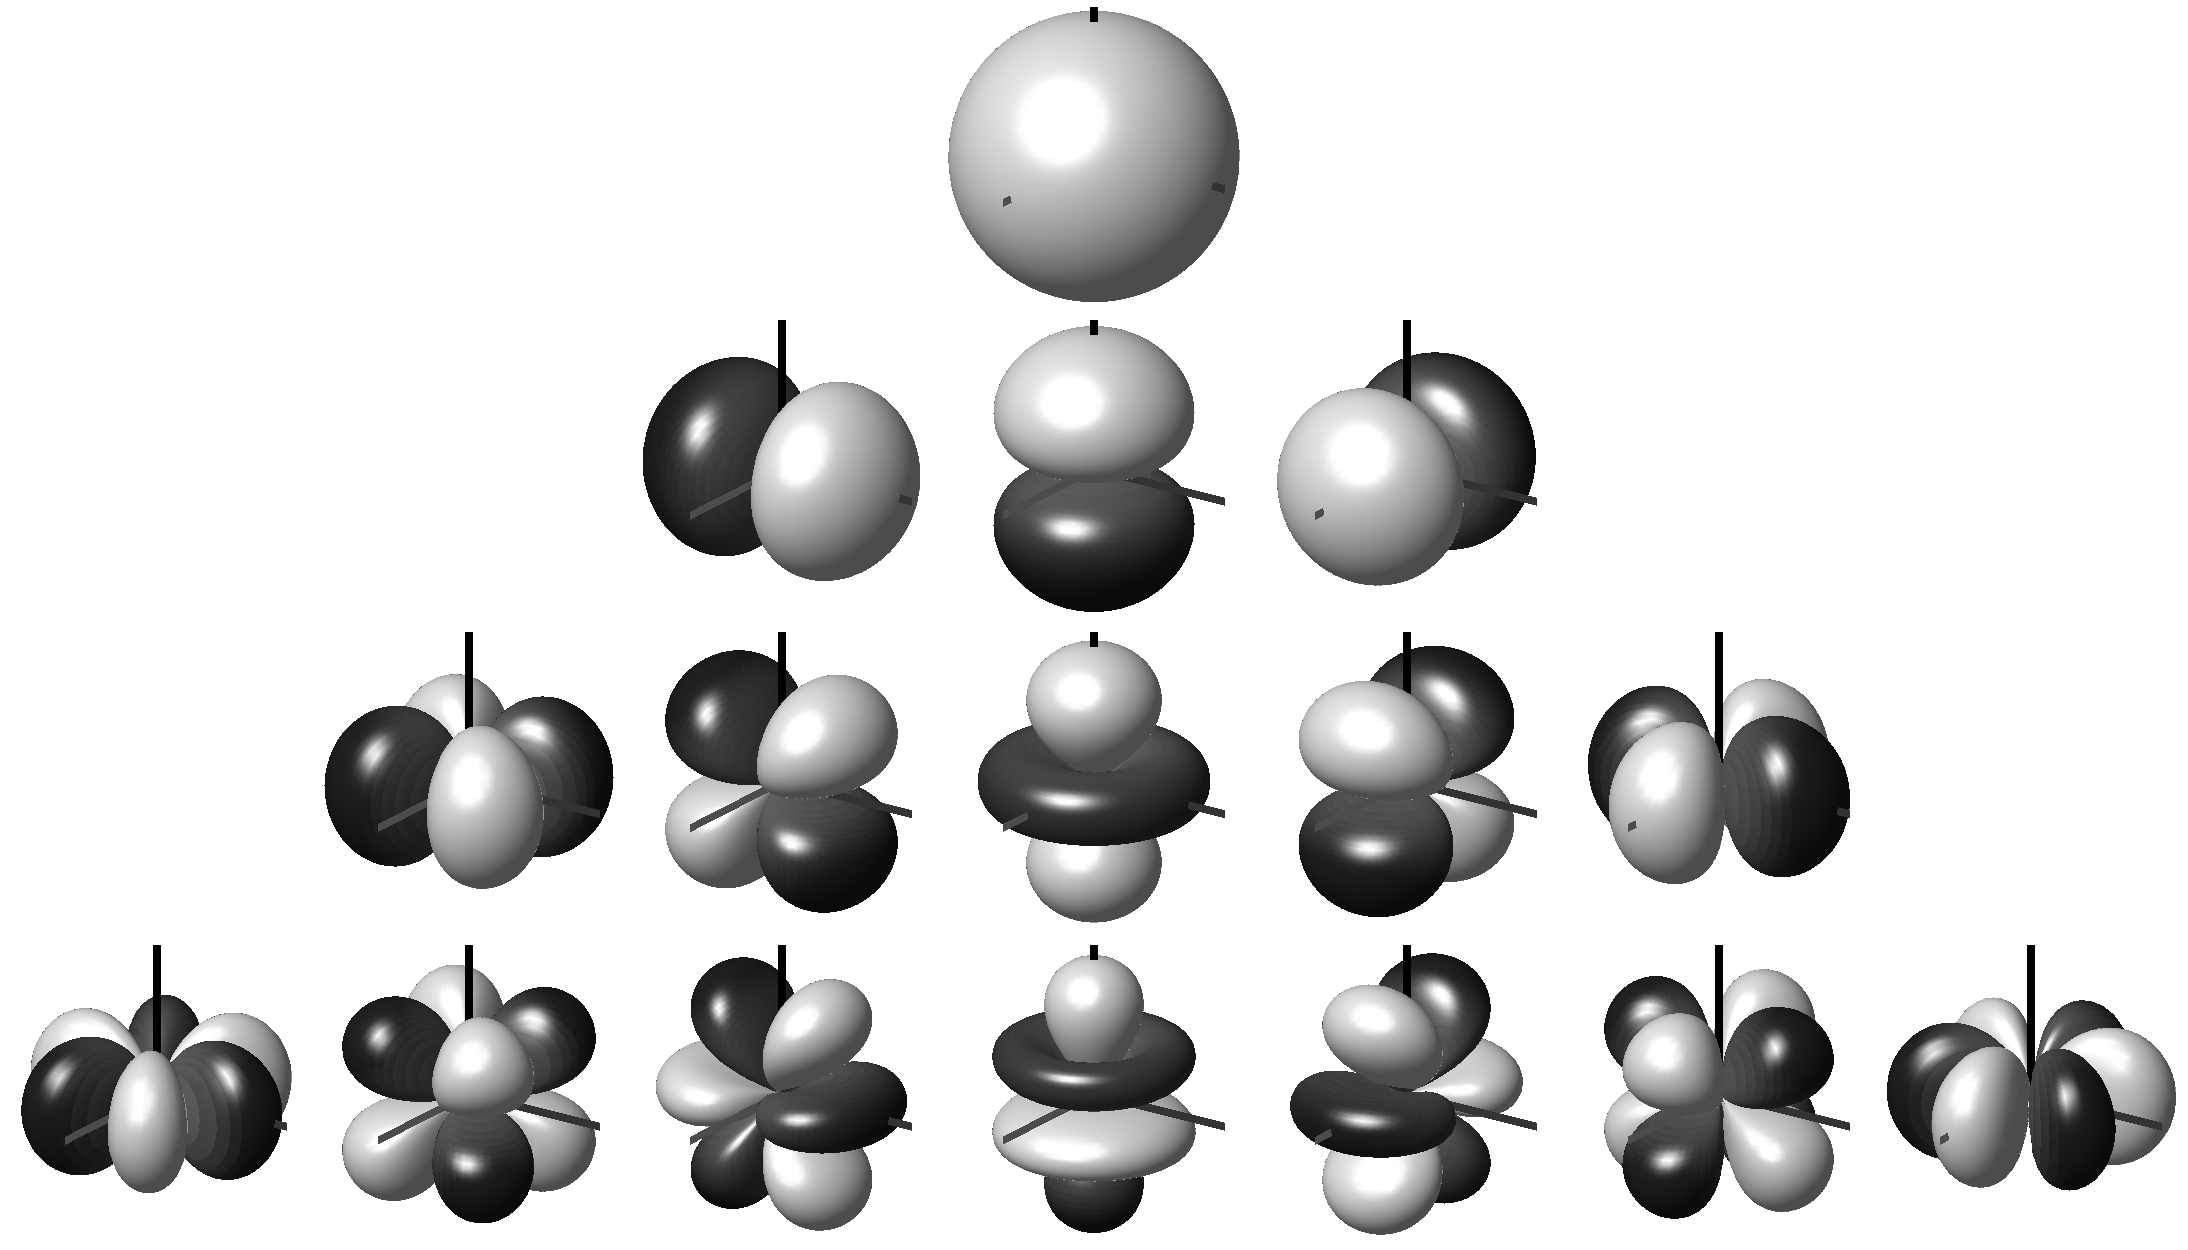
\includegraphics[width=\textwidth]{Figures/ScientificBackground/Spherical_Harmonics_deg3.png}
  \caption{Spherical harmonics up to order $N=3$. The rows correspond to the spherical harmonics of a given order $n$, and the columns span all possible degree values.}
  \label{fig:sphericalharmonics}
\end{figure}


\subsection{Spherical array processing}

Let us consider a sound field captured with a spherical microphone array, which contains $Q$ capsules distributed around a spherical surface of radius $R$ at the positions $\Omega_q, 1 \leq q \leq Q$. 
The captured frequency-domain signals $X_q(k)$ can be represented as the spherical harmonic domain signals $X_n^m(k)$ through the spherical harmonic transform of order $n$ and degree $m$ \cite{moreau20063d}:

\begin{equation}
	X_n^m(k) = \sum_{q=1}^{Q} X_q(k) Y_n^m(\Omega_q) \Gamma_n(kR),
	\label{eq:a2b}
\end{equation}
\todo{is that actually valid? or Y should be the complex-valued spherical harmonics?}

where the term $\Gamma_n(kR)$ models the radial transfer function, and depends on a number of factors, being the \textit{sphere configuration} one of the most prominent considerations. 
Sphere configuration, in its basic form, refers to the physical properties of the baffle where the capsules are mounted, and it can be either \textit{open} or \textit{rigid}. 
While open configuration is the simplest solution, it might present numerical problems in the form of zeros in its frequency response. Conversely, a rigid baffle interferes with the sound field and might create undesired interferences, but it improves the numerical condition from the open case. Fig.~\ref{fig:magnitude_kr} shows the simulated magnitude response of $\Gamma_n(kR)$  for a spherical array considering both configurations. 
The reader is referred to \cite{moreau20063d} and \cite{rafaely2004analysis}  for a deeper insight into the topic of spherical microphone array design.

%\begin{figure}[h!]
%  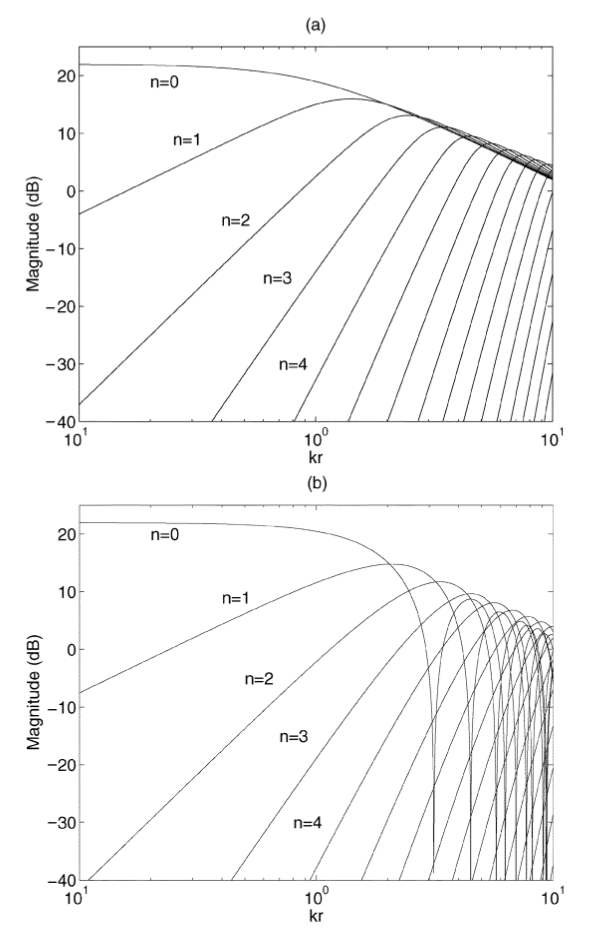
\includegraphics[width=\textwidth]{Figures/ScientificBackground/magnitude_kr.png}  
%  \caption{Magnitude of $\Gamma_n(kR)$ for different ambisonic orders, in the case of (a) rigid sphere, and (b) open sphere configurations. Adapted from \cite{rafaely2004analysis}. }
%  \label{fig:magnitude_kr}
%\end{figure}
%


\begin{figure}[hbt]
\begin{center}
  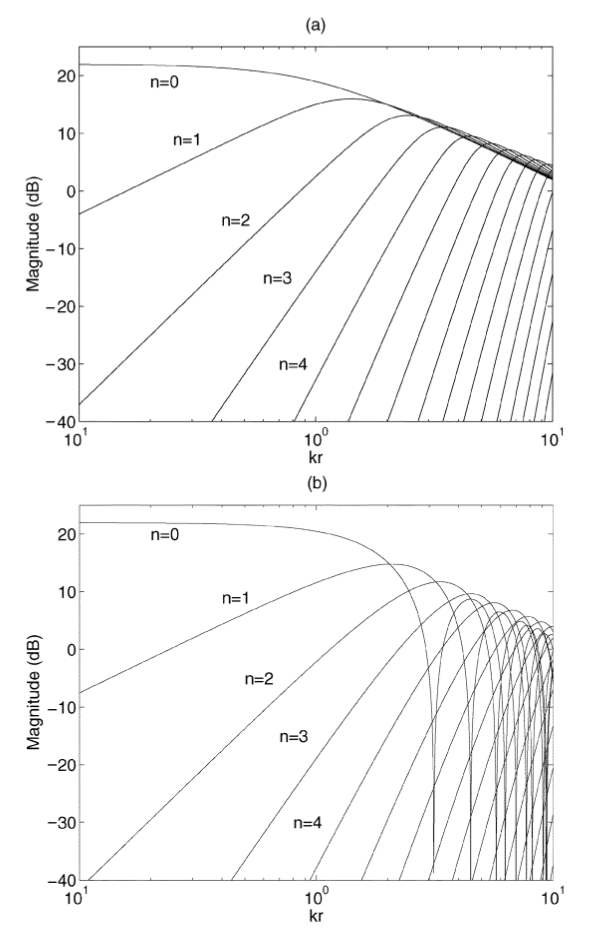
\includegraphics[width=0.5\textwidth]{Figures/ScientificBackground/magnitude_kr.png}
  \caption{Magnitude of $\Gamma_n(kR)$ for different ambisonic orders, in the case of (a) rigid sphere, and (b) open sphere configurations. Adapted from \cite{rafaely2004analysis}. }
	\label{fig:magnitude_kr}
	\end{center}
\end{figure}



%and depends on the microphone geometry, the directivity of the capsules and the physical properties of the baffle where the capsules are mounted.
%
% There are several possible sampling schemes of capsules along the sphere, each one having different properties; the reader is referred to  \cite{rafaely2004analysis} for a deeper insight. \\

By using the model from Eq.~\ref{eq:a2b}, the maximum spherical harmonic order $N$ that can be retrieved with negligible spatial aliasing depends on the number of microphone capsules \cite{moreau20063d}:
\begin{equation}
	N \geq (Q + 1)^2.
\end{equation}

Furthermore, the sphere radius $R$ has also an effect on the operational bandwidth of the microphone. According to \cite{moreau20063d}, the maximum aliasing-free operational frequency of a spherical microphone array is given by:
\begin{equation}
	f_{max} = \frac{c} {2 R \gamma},
	\label{eq:falias}
\end{equation}

with $c$ being the sound speed, and $\gamma$ the maximum aperture angle between two capsules. 
It is important to notice the existence of a practical minimum frequency of the spherical microphone array, given by the low magnitude in low frequencies of high ambisonic order components, as shown in Fig.~\ref{fig:magnitude_kr}. 



\section{Ambisonics}
\label{sec:ambisonics}

\subsection{Ambisonics Theory}

Ambisonics is a spatial sound recording and playback technology initially developed during the 1970s \cite{gerzon1973periphony}, and further expanded into its modern formulation around the 2000s \cite{daniel2000representation}.  
Ambisonics is based on the idea of decomposing a sound field into its spherical harmonic representation. 

Originally, the decomposition was limited to first-order spherical harmonics, as the so-called \textit{First Order Ambisonics} (FOA); mainly because of practical limitations. The technique was later formalized for arbitrary spherical harmonic orders, known as \textit{Higher Order Ambisonics} (HOA).
In general, with the term \textit{ambisonics} we will be referring to the latter definition.\\

\subsubsection{Ambisonic encoding}

Let us consider a sound field composed of a point sound source $S$ located in far-field at the angular position $\Omega_s$. The sound pressure at the coordinate origin $P$ can be expressed in terms of the spherical harmonic expansion of order $N$ as: \todo{check equation, find references, how to explain the domain? extend also to multiple sources by superposition}
\begin{equation}
	P = \sum_{n=0}^{N} \sum_{m=-n}^{n} Y_n^m(\Omega_s) S
	\label{eq:encoding}
\end{equation}


The ordered set of values of all spherical harmonics up to order $N$, evaluated at the source position, is known as the \textit{ambisonic coefficients}:
\begin{equation}
	Y_n^m(\Omega_s) = [Y_0^0(\Omega_s), Y_1^{-1}(\Omega_s),  \ldots ,  Y_N^N(\Omega_s)]
	\label{eq:sphericalharmonicvector}
\end{equation}

Furthermore, the process of multiplying the signal $S$ by the ambisonic coefficients is known in the literature as the \textit{ambisonic encoding}. The resulting signal vector is usually referred to as the \textit{ambisonic} (or \textit{B-Format}) signal $S_n^m$:
\begin{equation}
	S_n^m = Y_n^m(\Omega_s) S
\end{equation}


Although the term \textit{B-Format} was initially introduced as an alternative name for first-order ambisonic signals [gerzon, tesis de daniel], it is nowadays common to use it as a synonim of ambisonic signals, without any order restriction. We will use the latter acception in what follows.

Historically, the name \textit{B-Format} was used as an opposite of \textit{A-Format}, which describes the signals recorded by a tetrahedral microphone array \cite{gerzon1975design}. The tetrahedron is the simplest and most common form of spherical microphone arrays (indistinctly referred to as ambisonic microphones) with uniform capsule distribution. Again, the term \textit{A-Format} is also currently employed for referring to the signals recorded by any spherical microphone array, regardless of the number or arrangement of capsules.

Likewise, the process of signal conversion from the spatial domain (microphone capsules) to the spherical harmonic domain (ambisonic signals), as in Eq.~\ref{eq:a2b}, is known as \textit{A-B conversion}. A number of different approaches have been developed for this process, and the interested reader is referred to \cite{moreau20063d} for more information.

In practice, there are two alternative ways to generate ambisonic signals. The first one is the \textit{synthesis}, based on the direct application of ambisonics encoding (Eq.~\ref{eq:encoding}) to a monophonic signal. The second one is the \textit{recording} with a spherical microphone array, followed by the aforementioned domain conversion. \\


\subsubsection{Ambisonic Decoding}
Conversely, the sound field reconstruction is performed by the \textit{ambisonic decoding} operation. This process is equivalent to weight-and-sum beamforming in the spherical harmonic domain, and it is sometimes also referred to as the \textit{virtual microphone} technique \cite{zotter2019ambisonics}.

Let us consider a loudspeaker located at the angular position $\Omega_p$. In accordance with Eq.~\ref{eq:encoding}, the signal feed $P$ is \textit{decoded} from the ambisonic signal as:
\begin{equation}
	P = \sum_{n=0}^{N} \sum_{m=-n}^{n} Y_n^m(\Omega_s) S Y_n^m(\Omega_\ell)  \alpha_n 
	\label{eq:decoding}
\end{equation}

where $\alpha_n$ is a weighting factor which accounts for the beam directivity.
There are several standard weightings used for different purposes; their values are shown in Table~\ref{tab:alpha}, and the first-order directive patterns are plotted in Figure~\ref{fig:alpha}.

\begin{table}[t]
\caption{Ambisonic decoding: standard values of $alpha_n$ weightings. Adapted from \cite{daniel2000representation}.}
\begin{center}
\begin{tabular}{cccccc}
\toprule
Decoding & $N$ & \multicolumn{4}{c}{$n$} \\ 
&  & 0 & 1 & 2 & 3 \\
\midrule
\textit{basic} & 0 & 1  \\
	& 1 & 1 & 1  \\
 	& 2 & 1 & 1 & 1 \\
 	& 3 & 1 & 1 & 1 & 1 \\
\midrule
\textit{max-rE} & 0 & 0.577  \\
	& 1 & 0.775 & 0.4  \\
 	& 2 & 0.861 & 0.612 & 0.305 \\
 	& 3 & 0.906 & 0.732 & 0.501 & 0.246 \\
\midrule
\textit{in-phase} & 0 & 0.333  \\
	& 1 & 0.5 & 0.1  \\
 	& 2 & 0.6 & 0.2 & 0.029 \\
 	& 3 & 0.667 & 0.286 & 0.071 & 0.008 \\
\bottomrule
\end{tabular}
\label{tab:alpha}
\end{center}
\end{table}

\begin{figure}[htbp]
	\begin{center}
	\begin{minipage}[b]{0.9\linewidth}
		\centerline{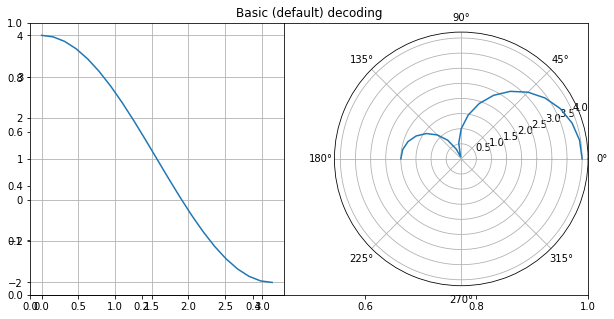
\includegraphics[width=\textwidth]{Figures/Introduction/basic.png}}
	\end{minipage}
	\begin{minipage}[b]{0.9\linewidth}
		\centerline{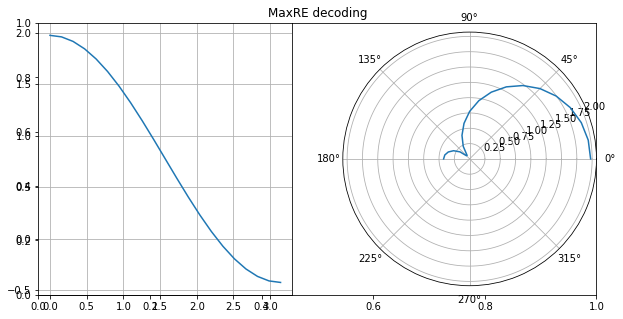
\includegraphics[width=\textwidth]{Figures/Introduction/maxre.png}}
	\end{minipage}
		\begin{minipage}[c]{0.9\linewidth}
		\centerline{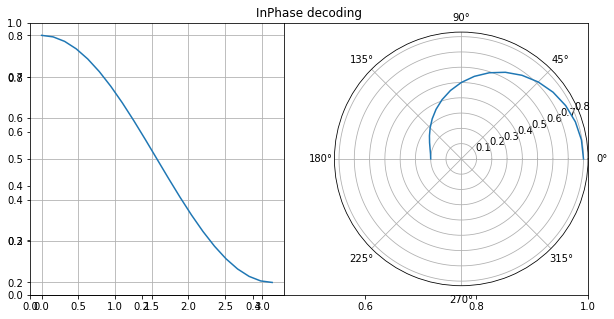
\includegraphics[width=\textwidth]{Figures/Introduction/inphase.png}}
	\end{minipage}
	\caption{Directive patterns of first-order ambisonic decoding.}
	\label{fig:alpha}
	\end{center}
\end{figure}


The decoding equation \ref{eq:decoding} can be written in matrix form as:
\begin{equation}
	P = S_n^m {Y_n^m (\Omega_p)}^T \alpha_n
\label{eq:decodingequation}
\end{equation}

where the superscript $T$ represents the matrix transposition. 
This equation can be extended to the usual case of decoding to a loudspeaker array, comprised of $L$ loudspeakers located at the positions $\Omega_L = [\Omega_{p_1}, \ldots, \Omega_{p_L}]$ . In such case, the loudspeaker feed vector $P_L$ can be written as:
\begin{equation}
	P_L = S_n^m D,
\label{eq:decodingequation2}
\end{equation}
where 
\begin{equation}
	D = \text{diag}(\alpha_n) [{Y_n^{m}(\Omega_{p_1})}^T, \ldots, {Y_n^{m}(\Omega_{p_L})}^T]
\end{equation}

is a $M \times L$ matrix known as the \textit{decoding matrix}, and $\text{diag}(\alpha_n)$ is a diagonal matrix of size $M$ containing the values of $\alpha_n$ along the main diagonal. 
Although the matrix $D$ is frequency-independent and depends solely on the loudspeaker array geometry, in practical scenarios it is usual to include frequency-dependent weightings, $\alpha_n(k)$, to improve the broadband sound field reconstruction \cite{daniel2000representation}.

Furthermore, sound field reconstruction with Eq.~\ref{eq:decodingequation2} is only possible when the loudspeakers are evenly located on the 3D space; in other words, the speaker layout must take the form of one of the five \textit{Platonic solids}: tetrahedron, cube, octahedron, dodecahedron or icosahedron.
Provided that this condition is usually difficult to fulfil in real scenarios, there are several methods which allow ambisonic decoding for such \textit{irregular} layouts. One of the most commonly used is the AllRAD method \todo{cite zotter}. AllRAD proposes a two step decoding: first, the ambisonic signal is decoded to a nearly-uniform layout of virtual speakers. Then, the signals of the virtual speakers are further distributed into the real speakers by the \textit{Vector-Based Amplitude Panning (VBAP)} method \todo{cite pulkki}.


% The reader is referred to [zotter? daniel? idhoa?] for more information about the vast field of study of ambisonic decoding.






\subsection{Practical considerations}

Due to historical and practical reasons, there are two aspects that must be taking into account when working with ambisonic signals: \textit{channel normalization} and \textit{channel ordering}. 
In the following, the term \textit{channels} will be used as a synonym for spherical harmonics, as they are usually referred to in sound engineering contexts\footnote{In fact, ambisonic signals are inherently multichannel, even though each channel corresponds to a spherical harmonic, and not to a loudspeaker feed as in traditional \textit{channel-based} audio.}.  \\


\subsubsection{Channel normalization}
Let us consider the spherical harmonics $Y_n^m(\Omega)$ as defined in Eq.~\ref{eq:sphericalharmonics}. Due to the orthonormal property showed in Eq.~\ref{eq:orthonormality}, they follow the \textit{fully 3d normalized} or \textit{N3D} channel normalization convention. \todo{what about the 1/sqrt(4pi)???}. 

Alternatively, the \textit{Schmidt 3d semi-normalized} or \textit{SN3D} [daniel] convention is also of widespread usage. The conversion between \textit{N3D} and \textit{SN3D} is driven by the following expression:
\begin{equation}
	{Y_n^m(\Omega)}^{\text{(N3D)}} = \sqrt{2n+1} {Y_n^m(\Omega)}^{\text{(SN3D)}}
\end{equation}

\textit{MaxN} is another existing convention. It defines all spherical harmonics as having a maximum absolute value of 1: 
\begin{equation}
	\max_{\Omega} |{Y_n^m(\Omega)}^{\text{(MaxN)}}| = 1, \forall (n, m)
\end{equation} 

Finally, the \textit{Furse-Malham} (or \textit{FuMa}) normalization only differs from \textit{Max-N} in the scaling of the zero-th order component: 
\begin{equation}
	{Y_n^m(\Omega)}^{\text{(FuMa)}} = \begin{cases}
		1 / \sqrt{2},  &\text{if } n = 0,\\
		{Y_n^m(\Omega)}^{\text{(MaxN)}},  &\text{else}.
	\end{cases}	
\end{equation} 

Each of the normalization schemes has its own particularities. For instance, \textit{N3D} is the most mathematically straightforward, and spherical harmonics defined in that way can be directly used for both encoding and decoding (as in Eqs~\ref{eq:encoding} and Eq.~\ref{eq:decoding}) -- however, from a sound engineer point of view, other normalization schemes with maximum values below the unity might be preferred, such as \textit{SN3D}. Besides this, \textit{FuMa} has been historically the default normalization \cite{gerzon1985ambisonics}, while the more modern \textit{N3D} and \textit{SN3D} were popularized after \cite{daniel2000representation}. \\

\begin{figure}[hbt!]
  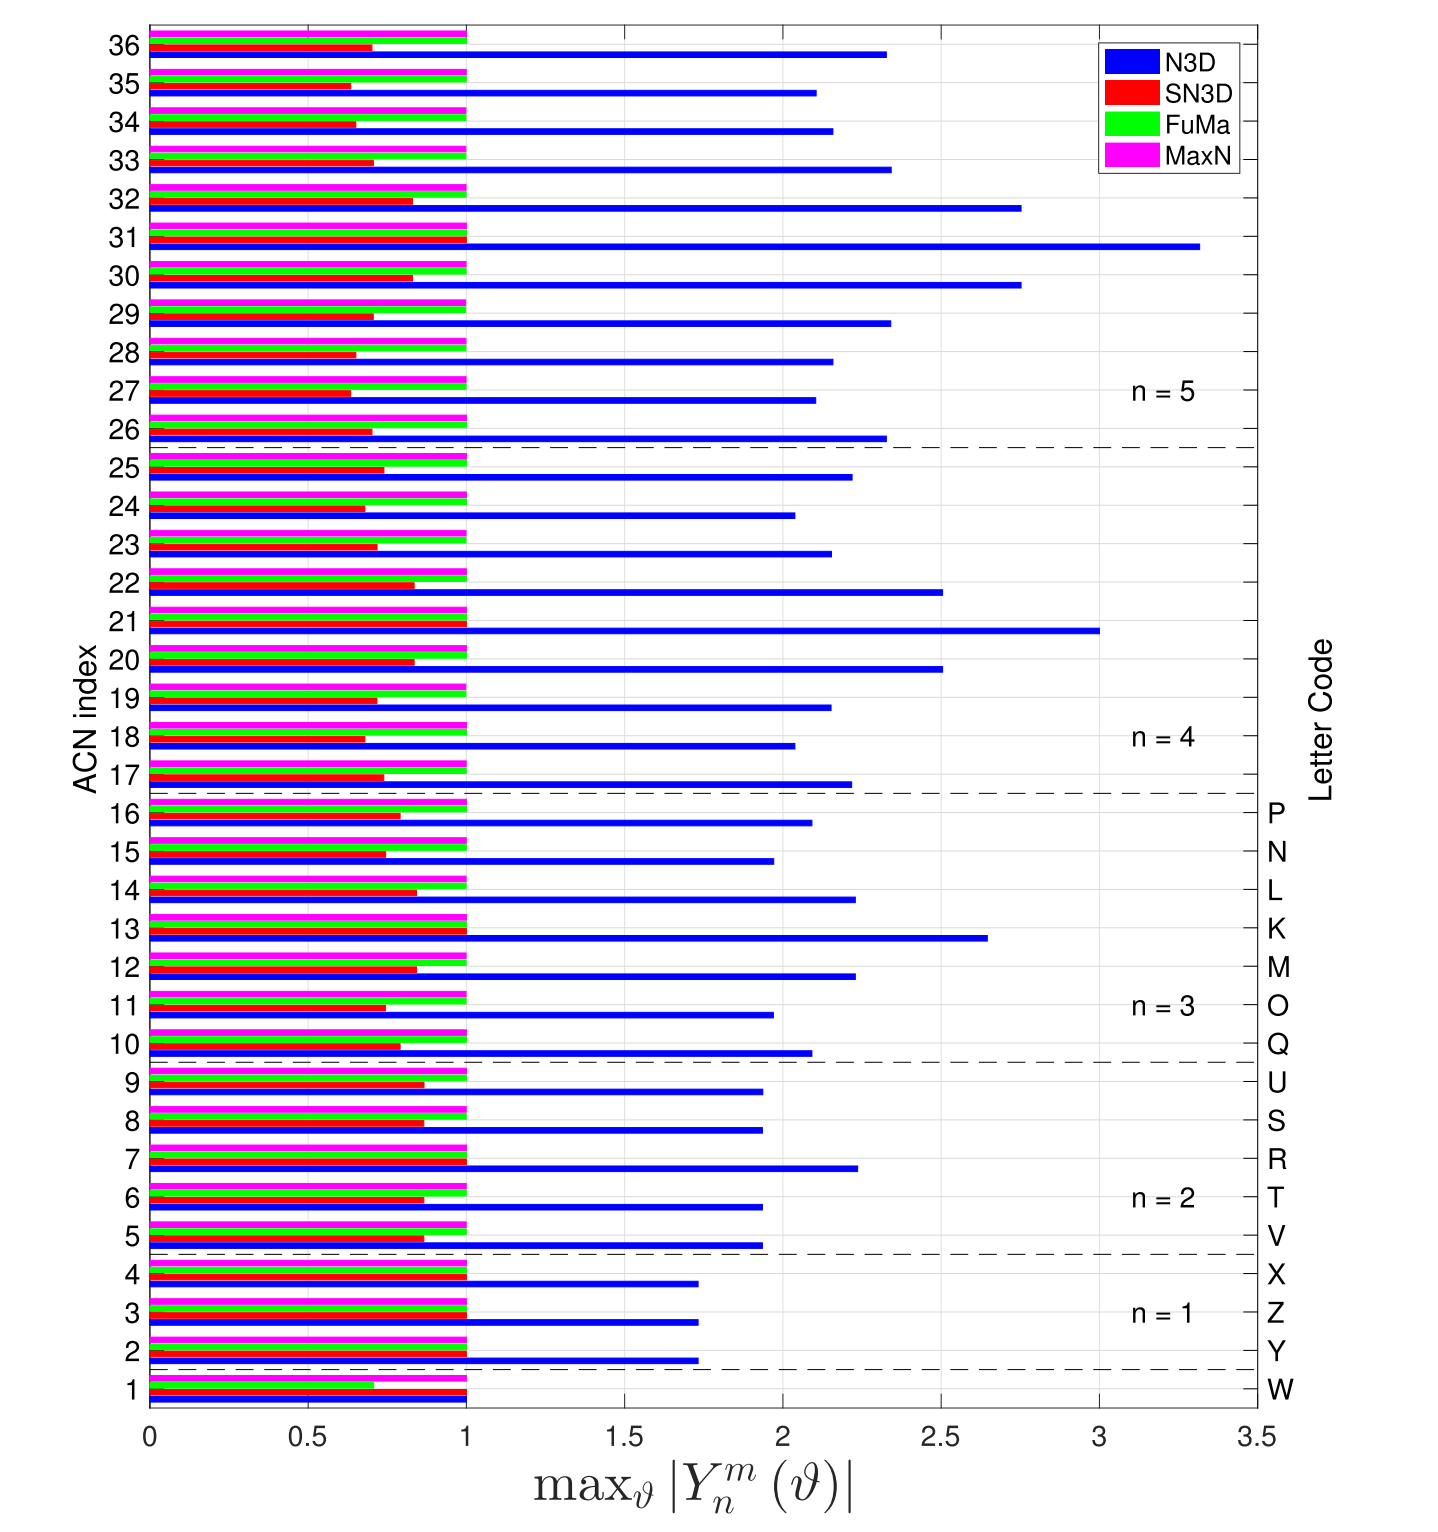
\includegraphics[width=\textwidth]{Figures/ScientificBackground/normalization.png}
  \caption{Maximum value of each ambisonic channel up to order 5, for all different normalization schemes. Image from \cite{carpentier2017ambisonic}.}
  \label{fig:normalization}
\end{figure}


As a summary, Figure~\ref{fig:normalization} displays the different normalization schemes. The reader is referred to \cite{carpentier2017ambisonic} for an extensive review on the topic.



\subsubsection{Channel ordering}

Channel ordering refers to the manner in which spherical harmonics, inherently organized in the 2D space by dimensions $n$ and $m$, are sorted into a one-dimensional vector. 

The \textit{ACN} (from \textit{Ambisonic Channel Number}) scheme follows from the mathematical description given in Eq.~\ref{eq:sphericalharmonicvector}. The spherical harmonics are first ordered by ascending order $n$ and, inside each order, by ascending degree $m$. The index of a given channel $i \in [0 \ldots M-1]$ can be thus obtained by the following relationship:
\begin{equation}
	i = n^2 + n + m 
\end{equation}

Historically, first-order ambisonic audio has followed what it might be called \textit{traditional B-Format} channel ordering \cite{gerzon1985ambisonics}. 
By this scheme, the four channels of a FOA signal $S_n^m$ are referred to by the axis where the corresponding spherical harmonic steers, plus the name $W$ for the zeroth order component:
\begin{equation}
	{S_n^m(\Omega)}^{\text{(FuMa CO)}} = [W, X, Y, Z]
\label{eq:fumaordering}
\end{equation}
where:
\begin{equation}
\begin{aligned}
	&W = S_0^0(\Omega) \\
	&X = S_1^1(\Omega) \\
	&Y = S_1^{-1}(\Omega) \\
	&Z = S_1^0(\Omega)
\end{aligned}	
\end{equation}

This nomenclature was extended to second and third order, and is currently known as the \textit{Furse-Malham} or \textit{FuMa} channel ordering. The channel names use all english alphabet letters from K to Z in third order and, although there would be enough letters to go up to fourth order, the unconvenience of the system was clear \cite{malham2003higher}.
Figure~\ref{fig:normalization} shows the equivalence between \textit{FuMa} (\textit{"letter code"}) and \textit{ACN} channel names.\\


In practice, there exist two main combinations of channel normalization and ordering schemes:
\begin{itemize}
  \item The \textit{classical} approach, usually limited to first-order ambisonics, which uses \textit{FuMa} normalization and channel ordering\footnote{In general, it may be expected that \textit{early} ambisonic material follow these conventions without any explicit mention to them.}.
  \item The \textit{modern} approach, inspired by the \textit{ambix} file format [cite ambix], with \textit{SN3D} normalization and \textit{ACN} channel ordering.
\end{itemize}

Anyhow, the \textit{classical B-Format} channel naming and ordering is still widely used when referring to first-order ambisonics. 
%In what follows, we will use indistinctly both \textit{classical} and \textit{ACN} conventions. \todo{is that true?}


\section{Parametric Spatial Audio Analysis}

Trough parametric analysis, sound fields may be described in terms of a small amount of sound sources and associate parameters. Such representation might reduce to a great extent the complexity of processing methods \cite{jarrett2017theory}.

One of the most successful sound field parametric models is DirAC \cite{Pulkki07}, which was originally conceived as a method for impulse response processing and spatial sound reproduction \cite{merimaa2005spatial}.

DirAC (acronym for \textit{Directional Audio Coding}) is a perceptually motivated time-frequency (TF) domain method, based on the assumption that any sound field may be reproduced with high perceptual quality by considering two parameters: the sound field diffuseness and the most prominent sound \textit{Direction-of-Arrival} (DOA) \cite{pulkki2018parametric}. \\



Let us consider a \textit{SN3D}-normalized first-order ambisonic signal in time-frequency domain, $S_n^m(k, n)$. 
For the sake of clarity, we will use in this section \textit{FuMa} channel notation and ordering (Eq.~\ref{eq:fumaordering}):
\begin{equation}
	S_n^m(k, n) = [W(k, n), X(k, n), Y(k, n), Z(k, n)]
\end{equation}

Given this representation, we can express the \textit{pressure} $P(k,n)$ of the sound field as:
\begin{equation}
	P(k,n) = W(k,n)
\end{equation}
as well as the sound \textit{pressure-gradient} (or \textit{velocity}) $\pmb{U}(k,n)$ as: 
\begin{equation}
	\pmb{U}(k,n) = - \frac{1}{\rho_0 c} [X(k, n), Y(k, n), Z(k, n)], 
\end{equation}
where $\rho_0$ is the mean density of the medium, and $c$ is the speed of sound.\\ 

The \textit{active intensity} $\pmb{I}(k,n)$, defined as the amount of transmitted acoustic energy, can be expressed in terms of sound pressure and velocity \cite{fahy1990sound}:
\begin{equation}
	\begin{aligned}
	\pmb{I}(k,n) &=  \Re\{P^*(k,n)\pmb{U}(k,n)\} \\
	&= - \frac{1}{\rho_0 c}\Re\{W^*(k,n)[X(k,n),Y(k,n),Z(k,n)]\},
	\end{aligned}
\end{equation}
where $^*$ represents the complex conjugate operator. \\

An estimate of the instantaneous DOA $\Omega(k,n)$ can be extracted from the intensity vector, interpreting each of its time-frequency bins as a point in the cartesian space. Effectively, the sound propagation direction is the opposite to the observed arrival direction. 
\begin{equation}
	\Omega(k,n) = \angle(-\pmb{I}(k,n)),
\label{eq:doa}
\end{equation}
with $\angle$ representing the spherical angle operator of a cartesian vector. The result of this computation must be understood as the direction of the net energy flow, which in the case of a single plane-wave will correspond to the source position. \\

Another useful parameter is the \textit{energy density} $E(k,n)$ \cite{stanzial1996reactive}:
\begin{equation}
	\begin{aligned}
		E(k,n) &= \frac{1}{2\rho_0 c^2} |P(k,n)|^2 + \frac{1}{2} {\|\pmb{U}(k,n)\|^2} \\
		&=  \frac{1}{2\rho_0 c^2} \Big(|W(k,n)|^2 + \| [X(k,n), Y(k,n), Z(k,n)] \|^2\Big).
	\end{aligned}
	\label{eq:energydensity}
\end{equation}\\

Finally, the \textit{diffuseness} $\Psi(k,n)$ can be computed from the sound intensity and  energy density \cite{merimaa2005spatial}:
\begin{equation}
	\begin{aligned}
		\Psi(k,n) &= 1 - \frac{ \| \langle \pmb{I}(k,n) \rangle \| }{ c \langle E(k,n) \rangle } \\
		&= 1 - 2\frac{ \| \langle \Re\{W^*(k,n)[X(k,n),Y(k,n),Z(k,n)]\} \rangle \| }{ \langle |W(k,n)|^2 + \| [X(k,n), Y(k,n), Z(k,n)] \|^2 \rangle },
	\end{aligned}
\label{eq:psidefinition}
\end{equation}
 
 where the symbols $\langle \cdot \rangle$ represent the expectation operator, which is usually implemented as time-domain averaging. 

Even though Eq.~\ref{eq:psidefinition} (known as \textit{DirAC's diffuseness}) is one of the most common ambisonic diffuseness estimators, several alternative formulations exist. 
Other diffuseness estimation procedures include the \textit{coefficient of variation method} \cite{ahonen2009diffuseness} and the more recent \textit{COMEDIE} estimator \cite{epain2016spherical}. 
In any case, in what follows, the term \textit{diffuseness} and the symbol $\Psi$ will refer by default to Eq.~\ref{eq:psidefinition}. 

As a mathematical convenience, we will define the \textit{B-Format coherence} as the complement of the diffuseness:
\begin{equation}
	\Delta(k,n) = 1 - \Psi(k,n) 
	\label{eq:delta}
\end{equation}

In conclusion, Figure~\ref{fig:dirac} plots the spectrograms of the DOA $\Omega(k,n)$ and diffuseness $\Psi(k,n)$ of a FOA recording, which consists of a sound source located at the front, plus a moderate amount of reverberation and background noise. 

\begin{figure}[h!]
	\begin{center}
	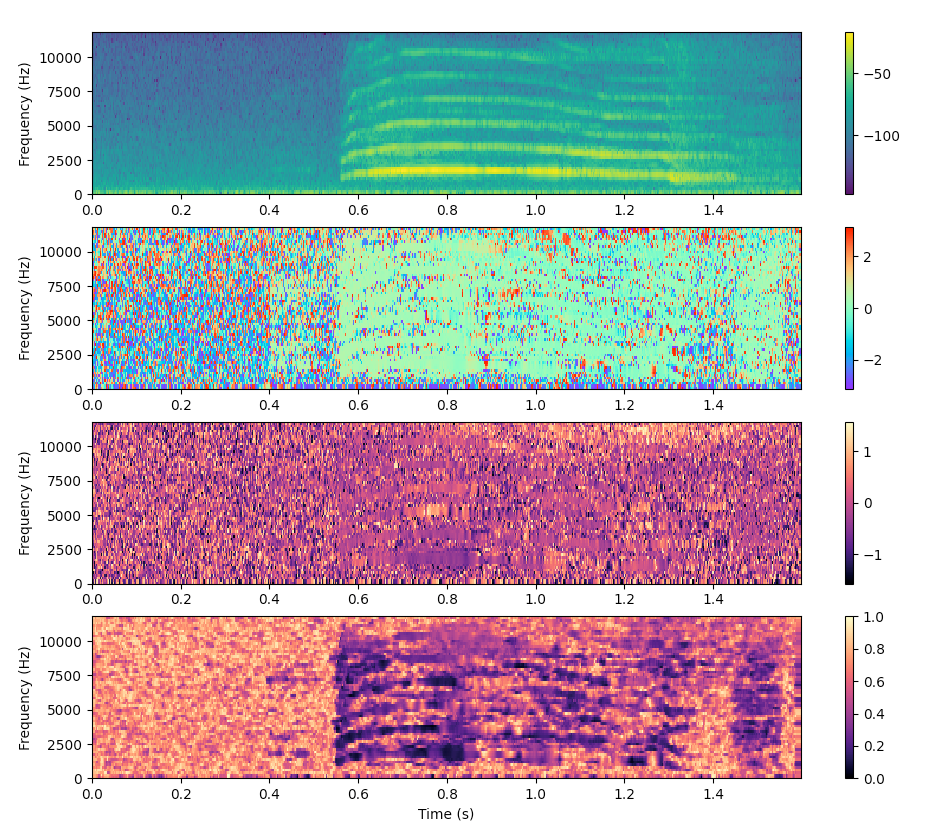
\includegraphics[width=\textwidth]{Figures/Introduction/spectrograms.png}
	\caption{Parametric time-frequency spatial audio analysis of a first order ambisonic recording. From top to bottom: 1.) Magnitude spectrogram of the omnidirectional channel. 2.) and 3.) Azimuth and elevation of the estimated instantaneous narrowband DOAs $\Omega(k,n)$. 4.) Instantaneous narrowband diffuseness $\Psi(k,n)$.}
	\label{fig:dirac}
	\end{center}
\end{figure}




\section{Spatial Coherence Analysis}
\todo{put this chapter in context or something}\\


In the context of microphone array signal processing, diffuseness is commonly estimated through the
\textit{Magnitude Squared Coherence} (MSC) \cite{elko_spatial_2001} between two frequency-domain signals $S_1$ and $S_2$, as a function of the
\textit{wavenumber} $k$ and the microphone distance $r$:
\begin{equation}
    \text{MSC}_{12}(k r) =
	\frac{|\left\langle S_1(k r) S_2(k r)^* \right\rangle|^2}
	{\left\langle|S_1(k r)|^2\right\rangle \left\langle|S_2(k r)|^2\right\rangle},
    \label{eq:MSC}
\end{equation}
where the $\left\langle \cdot \right\rangle$ operator represents the temporal
expected value, and $^*$ defines the complex conjugate operator. In the case of spherical isotropic noise fields, Eq.~(\ref{eq:MSC})
can be expressed in terms of microphone directivity patterns
$T(\phi,\theta,k r)$ as \cite{elko_spatial_2001}:

\begin{equation}
	\begin{aligned}
&\text{MSC}_{12}(k r) = \frac{|N_{12}(k r)|^2}{|D_{12}(kr)|^2} \\
&= \frac{|\int_{0}^{\pi} \int_{0}^{2\pi} T_1(\phi,\theta,k r) T_2^*(\phi,\theta,k r) e^{-jk r cos\theta} sin\theta d\theta d\phi|^2}{|\sqrt{ \int_{0}^{\pi} \int_{0}^{2\pi} |T_1(\phi,\theta,k r)|^2 sin\theta d\theta d\phi } \sqrt{\int_{0}^{\pi} \int_{0}^{2\pi}|T_2(\phi,\theta,k r)|^2 sin\theta d\theta d\phi}|^2}.
\label{eq:MSCdir}
    \end{aligned}
\end{equation}


Moreover, the general expression of the directivity of a first-order differential microphone is given by the following relationship:

\begin{equation}
	\begin{aligned}
	T_i(\Omega_i) = \alpha_i + (1 - \alpha_i) \cos{\Omega_i},
	\end{aligned}
\end{equation}


where $i \in [1,2]$ is the microphone index, $\Omega_i$ is the angle between wave incidence and microphone orientation axis, and $\alpha_i \in [0,1]$ is the directivity parameter of the microphone $i$, which ranges from bidirectional ($\alpha_i = 0$) to omnidirectional ($\alpha_i = 1$). \\


For first-order differential microphones, there is a closed-form expression for the numerator and denominator of Eq.~(\ref{eq:MSCdir}):
\begin{equation}
	\begin{aligned}
    &N_{12}(k r) =  \frac{\alpha_1 \alpha_2 sin(kr)}{kr} \\
    &+ \frac{(1-\alpha_2)(1-\alpha_2)(x_1x_2+y_1y_2)}{(kr)^3}(sin(kr)-kr cos(kr)) \\
    &+ \frac{z_1 z_2}{kr^3}[ ( (kr)^2 sin(kr) + 2kr cos(kr) )(1-\alpha_1)(1-\alpha_2) 
    + 2 sin(kr)(1-\alpha_1)(1-\alpha_2) ] \\
    &+ \frac{z_1}{(kr)^3}[ j(kr)^2 \alpha_2 cos(kr)(\alpha_1-1) + jkr \alpha_2 sin(kr)(1+\alpha_1) ] \\
    &+ \frac{z_2}{(kr)^3}[ j(kr)^2 \alpha_1 cos(kr)(\alpha_2-1) + jkr \alpha_1 sin(kr)(1+\alpha_2) ],\\
    &D_{12}(kr) =  \frac{\sqrt{3 \alpha_1^2+(1-\alpha_1)^2}\sqrt{3 \alpha_2^2+(1-\alpha_2)^2}}{3},
    \label{eq:closedform_msc}
    \end{aligned}
\end{equation}
where $x_i$, $y_i$ and $z_i$ are the cartesian coordinates of the wave incidence angle $\Omega_i$. \todo{check}.





\section{Reverberation}

In the context of room acoustics, reverberation refers to \textit{"the energy of a sound source that reaches a listener indirectly, by reflecting from surfaces within the surrounding space occupied by the sound source and the listener"} \cite{begault20003}. 
Conversely, in anechoic or free-field conditions, where reverberation is not present, only the direct path of the sound source exists.
Assuming linearity and time-invariance, room reverberation can be fully characterised by its impulse response (IR). \\

Reverberation models often consider two differentiated parts of the reverberant tail, based on both physical and perceptual characteristics: the \textit{early reflections} and the \textit{late reverberation}. 
Early reflections, as the name suggests, refers to the individual sound paths arriving to the listener after a few reflections on the room surfaces, which cause some degree of attenuation. Early reflections typically arrive with a time difference between 1 and 80 ms after the direct path \cite{begault20003}. 
The term late reverberation encompasses all sound paths arriving to the listener after many reflections. Since the temporal density of such reflections increases with time, late reverberation is often modelled in statistical terms.
An schematic representation of a room impulse response (RIR) is shown in Figure~\ref{fig:rir}.\\

\begin{figure}[htbp]
	\begin{center}
	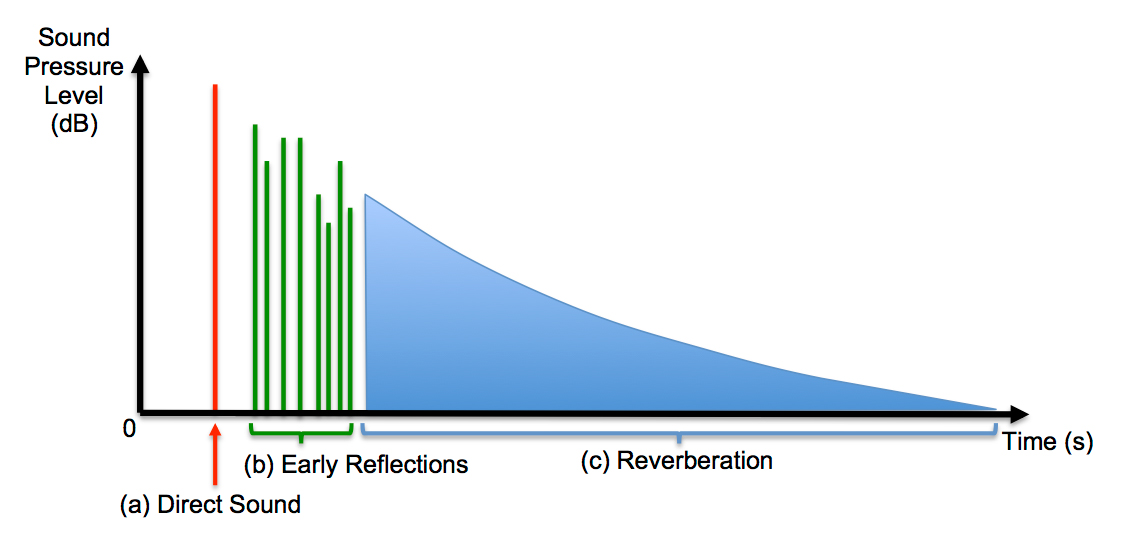
\includegraphics[width=\textwidth]{Figures/Introduction/Acoustic_room_impulse_response.jpg}
	\caption{Room impulse response model, from \cite{murphy2017acoustic}.}
	\label{fig:rir}
	\end{center}
\end{figure}

By following this model, a RIR $h(t)$ can be described as a sequential combination of responses:
\begin{equation}
	h(t) = h_D(t) + h_R(t),
\label{eq:directreverberant}
\end{equation}
where $h_D(t)$ and $h_R(t)$ represent the \textit{direct} (direct path plus early reflections) and \textit{reverberant} (late reverberation) components of the RIR. respectively.\\


The room impulse response is a function of both the source and the receiver locations. Different levels, delays and directions of direct path and early reflections can obtained from measurements in the same room. However, it is generally assumed that the late reverberation is fixed for a given room, regardless of source/receiver positions. \\

Room reverberation plays an important role in psychoacoustics. While early reflections are usually perceived together with the direct path as a single auditory event, due to the \textit{precedence effect} \cite{haas1972influence}, late reverberation has often an influence on the received signal. In the specific case of speech, late reverberation is associated with a loss of intelligibility \cite{braun2018speech}.
In the context of spatial perception, it has been shown that early reflections help the localization and externalization of sources \cite{rudrich2019improving}, while the late reverberation is associated with a spaciousness perception of the room \cite{begault20003}. \\


There are a number of measurable parameters which help to characterise room acoustics. 
Perhaps one of the most widespread is the \textit{reverberation time} $T_{60}$ \cite{kuttruff2016room}. It represents the time required for the reverberant sound field power to decay by 60 dB.
Reverberation time can be accurately computed from the room geometry \cite{sabine1927collected} or from the IR \cite{schroeder1965new}.

In the latter case, the $T_{60}$ value is usually estimated from the \textit{Energy Decay Curve} (EDC), which is defined as:

\begin{equation}
	\text{EDC}(t) = 10 \log_{10} \sum_{t'=t}^{\infty} h^2(t),
\end{equation}

where $h(t)$ represents the room impulse response. The values are normalized such that the maximum peak of the curve corresponds to 0 dB.

The EDC is usually modelled as a straight line in logarithmic scale. Therefore, the $T_{60}$ estimation is performed by estimating the slope of a straight line between two reference levels on the EDC time series.
Some of the most used reference levels receive specific names: \textit{Early Decay Time} (EDT), $T_{60}$, and reverberation times $T_{10}$, $T_{20}$ and $T_{30}$. Table\ref{tab:reverberationtimes} shows their correspondent reference levels, where the maximum energy peak is normalized to 0 dB. An schematic representation of the reference levels is depicted in Figure~\ref{fig:reverberationtimes}.

An alternative parameter is the \textit{decay rate} $\alpha_{60}$, which is related to reverberation time $T_{60}$ as:
\begin{equation}
	\alpha_{60} = \frac{3 \ln{(10)}} {T_{60}} (\text{dB/s}).
\end{equation}
 
The decay rate is thus the slope of the EDC curve, in logarithmic scale, expressed in dB per second.  

To conclude, it is important to notice that reverberation time is frequency-dependent. Accordingly, it is usual to report it for octave or third-octave bands, or alternatively to provide its value at a specific frequency. \\


\begin{table}[t]
\caption{Reverberation time computation: usual reference levels}
\begin{center}
\begin{tabular}{ccccc}
\toprule
   & $\text{EDT}$ & $T_{10}$ & $T_{20}$ & $T_{30}$ \\
\midrule
$L_{max} (dB)$ & 0 & -5 & -5 & -5  \\
$L_{min} (dB)$ & -10 & -15 & -25 & -35 \\
\bottomrule
\end{tabular}
\label{tab:reverberationtimes}
\end{center}
\end{table}

\begin{figure}[htbp]
	\begin{center}
	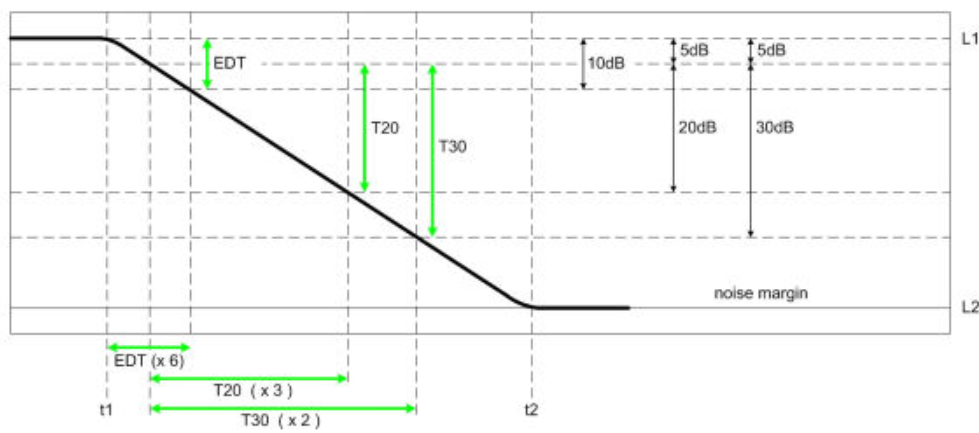
\includegraphics[width=\textwidth]{Figures/Introduction/edt.png}
	\caption{Room impulse response model, adapted from \url{http://www.bnoack.com/}.}
	\label{fig:reverberationtimes}
	\end{center}
\end{figure}


The \textit{Direct to Reverberant Ratio} (DRR) is another relevant acoustic parameter. DDR represents the ratio between direct and reverberant parts of the RIR, as defined in Eq.~\ref{eq:directreverberant}:
\begin{equation}
	DRR = 10 \log_{10} \frac{ \sum_{t=1}^{L_D} h^2_D(t) }{ \sum_{t=1}^{L_R} h^2_R(t)},
\end{equation}
with $L_D$ and $L_R$ as the length of the direct $h_D(t)$ and reverberant $h_R(t)$ filters, respectively.  
At a psychoacoustic level, the direct to reverberant ratio is one of the main cues for distance perception \cite{begault20003}. 

Since the direct path and early reflections (but not the late reverberation) depend on the relative position between source and receiver , the filter $h_D(t)$ and therefore the DRR are as well location-dependent. For a given room, the source-receiver distance that produces a DRR of 0 dB is known as the \textit{critical distance}. 


%\subsection{SOFA Conventions}
%
%The availability of recorded room impulse responses is of great importance to many acoustic signal processing problems. 
%As we have seen, many different RIRs can be obtained from the same room, by just varying the position of the source and the receiver; when the number of source and receiver positions increases, the total amount of measurements increases geometrically. 
%Besides that, the actual format and organisation of the produced data (not only the RIR themselves, but also the source/position annotations) can be arbitrarily different when produced by different groups of people.
%
%In order to overcome potential interoperatibility and reusability issues, the \textit{Spatially Oriented Format for Acoustics} (SOFA) convention \cite{majdak2013spatially}, also known as the \textit{AES-69} standard \cite{majdak2015aes69}, proposes a unified file format for the storage of IR-related data. 
%Despite that SOFA was initially created with a focus on \textit{Head-Related Impulse Response} (HRIR) data, its structure is very convenient to any kind of multi-location impulse responses, including ambisonics.


\todo{RIR SIMULATION: IMAGE METHOD}


\section{Signal Models}


Let us consider a sound source represented by the signal $s(t)$, located in a given acoustic enclosure characterised by its room impulse response $h(t)$. The resulting reverberant signal $x(t)$ can be therefore described as the \textit{convolutive mixture} of the source and the RIR: 
\begin{equation}
	x(t) = s(t) \ast h(t).
\label{eq:convolutivemixture}
\end{equation}

When dealing with multichannel room impulse responses, as it is the case in ambisonics, the multichannel reverberant signal $x_m(t)$ is obtained by the convolutive mixture of each RIR channel independently:
\begin{equation}
	x_m(t) = s(t) \ast h_m(t).
\label{eq:convolutivemixturemultichannel}
\end{equation}

The time domain convolution operation, under certain assumptions, is equivalent to the multiplication in frequency domain. By doing so, Eq.~\ref{eq:convolutivemixture} can be expressed as:
\begin{equation}
	X(k,n) = S(k,n) H(k,n).
\label{eq:multiplicativetransferfunction}
\end{equation}

Eq.~\ref{eq:multiplicativetransferfunction}, also known as the \textit{Multiplicative Transfer Function (MTF) model} is only valid when the length of the filter $h(t)$ is smaller than the length of the analysis window used in the STFT. 


On the contrary, when the filter $h(t)$ spans across several analysis windows, the resulting model is referred to as the \textit{Convolutive Transfer Function (CTF) model}:
\begin{equation}
	X(k, n) = \sum_{l=0}^{L_h-1} H(k, l) S(k, n-l), 
\label{eq:convolutivetransferfunction}
\end{equation} 
where $L_h$ is the length of the filter $H(k, n)$ in time frames. 



\todo{isotropic noise}



%\section{Practical Considerations}
% TODO I don't remember what is this

